\chapter{Bruggen \& Sluizen}
\vspace{-120px}
\question{1}{Bij welke brug is doorvaart toegestaan en is tegenliggende vaart verboden?}


\begin{figure}[H]
	\centering
	\begin{minipage}[b]{0.23\textwidth}
		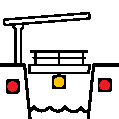
\includegraphics[width=\textwidth]{Hoofdstukken/Bruggen/pdf/brug_doorvaart_toegestaan.pdf}
		\centering
		A
	\end{minipage}
	\hfill
	\begin{minipage}[b]{0.23\textwidth}
		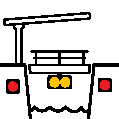
\includegraphics[width=\textwidth]{Hoofdstukken/Bruggen/pdf/brug_doorvaart_geen_tegenligger.pdf}
		\centering
		B
	\end{minipage}
	\hfill
	\begin{minipage}[b]{0.23\textwidth}
		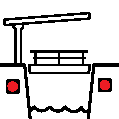
\includegraphics[width=\textwidth]{Hoofdstukken/Bruggen/pdf/brug_doorvaart_verboden.pdf}
		\centering
		C
	\end{minipage}
	\hfill
	\begin{minipage}[b]{0.23\textwidth}
		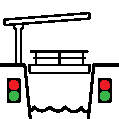
\includegraphics[width=\textwidth]{Hoofdstukken/Bruggen/pdf/brug_aanstonds_toegestaan.pdf}
		\centering
		D
	\end{minipage}
\end{figure}


\question{2}{Welke brug gaat bijna open?}

\begin{figure}[H]
	\centering
	\begin{minipage}[b]{0.23\textwidth}
		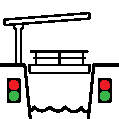
\includegraphics[width=\textwidth]{Hoofdstukken/Bruggen/pdf/brug_aanstonds_toegestaan.pdf}
		\centering
		A
	\end{minipage}
	\hfill
	\begin{minipage}[b]{0.23\textwidth}
		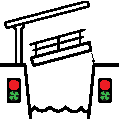
\includegraphics[width=\textwidth]{Hoofdstukken/Bruggen/pdf/brug_sluitend.pdf}
		\centering
		B
	\end{minipage}
	\hfill
	\begin{minipage}[b]{0.23\textwidth}
		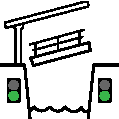
\includegraphics[width=\textwidth]{Hoofdstukken/Bruggen/pdf/brug_toegestaan.pdf}
		\centering
		C
	\end{minipage}
	\hfill
	\begin{minipage}[b]{0.23\textwidth}
		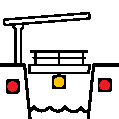
\includegraphics[width=\textwidth]{Hoofdstukken/Bruggen/pdf/brug_doorvaart_toegestaan.pdf}
		\centering
		D
	\end{minipage}
\end{figure}

\question{3}{Wat betekenen de groene borden op deze burg?}
\begin{figure}[H]	
	\vspace{-10px}
	\begin{minipage}[]{0.70\textwidth}
		\begin{enumerate}[topsep=0pt, label=\Alph*.]
			\item Brug buiten bediening
			\item Het gebied tussen de borden is het aangeraden vaargebied
			\item Doorvaart toegestaan
			\item Doorvaart toegestaan, tegenliggers mogelijk
		\end{enumerate}
	\end{minipage}
	\begin{minipage}[]{0.29\textwidth}
		\begin{figure}[H]
			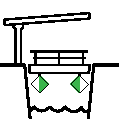
\includegraphics[width=0.80\textwidth,right]{Hoofdstukken/Bruggen/pdf/brug_aanbevolen_gebied.pdf}
		\end{figure}
	\end{minipage}
	\vspace{-10px}
\end{figure}

\question{4}{Wat betekent een enkele gele ruit?}
\answerTextFour{Doorvaart verboden}{Doorvaart toegestaan, tegenliggers mogelijk}{Doorvaart toegestaan, tegenliggers niet mogelijk}{Brug buiten bediening}

\question{5}{De brug gaat al naar beneden. Mag je er nog onder door varen?}
\begin{figure}[H]	
	\vspace{-10px}
	\begin{minipage}[]{0.70\textwidth}
		\begin{enumerate}[topsep=0pt, label=\Alph*.]
			\item Ja, het groene licht brandt nog
			\item Ja, zolang het nog past
			\item Nee, \textit{tenzij} je niet meer kan stoppen
			\item Nee, je mag nooit onder een sluitende brug door varen
		\end{enumerate}
	\end{minipage}
	\begin{minipage}[]{0.29\textwidth}
		\begin{figure}[H]
			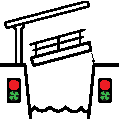
\includegraphics[width=0.80\textwidth,right]{Hoofdstukken/Bruggen/pdf/brug_sluitend.pdf}
		\end{figure}
	\end{minipage}
	\vspace{-10px}
\end{figure}
